\documentclass{article}
\usepackage{graphicx} % Required for inserting images
\title{D1: Analisi dei Requisiti}
\author{G06}
\usepackage{fancyhdr}
\usepackage{hyperref}
\usepackage{float}
\newcommand{\myheaderimage}{\includegraphics[width=2cm]{D3/Images/LogoEasyLib.png}}
\pagestyle{fancy}
\fancyhf{} % Clear the header and footer
\lhead{\myheaderimage} % Place the image in the top right corner
\setlength{\headheight}{3cm} % Adjust the height as needed
\rhead{D1-G06}

\begin{document}

\maketitle
\tableofcontents
\newpage



\section{Scopo del Documento}
Il presente documento riporta l’analisi dei requisiti di sistema del progetto di \textbf{EasyLib}, in linguaggio naturale.
Il suo scopo è quello di:
\begin{itemize}
    \item Presentare gli obiettivi del progetto;
    \item Definire i requisiti funzionali e non funzionali;
    \item Presentare i requisiti di Front-End;
    \item Presentare i requisiti di Back-End.
\end{itemize}

\section{Obiettivi del progetto}
Il progetto ha come fine quello di realizzare un’applicazione per la gestione di una biblioteca. In particolare applicazione permetterà:
\begin{itemize}
    \item \textbf{A.} Ad un utente autenticato, ovvero ad un utente provvisto di credenziali (mail e password) di poter:
        \begin{itemize}
            \item Controllare quali libri sono disponibili per il prestito e quali no
            \item Donare libri alla biblioteca
            \item Richiedere il prestito di un libro alla biblioteca
            \item Lasciare una valutazione del libro, una volta riconsegnato
        \end{itemize} 
    \item \textbf{B.} Ad un utente anonimo, cioè ad un utente il quale non ha ancora effettuato l’accesso al sistema, di poter:
        \begin{itemize}
            \item Registrarsi nel sistema.
            \item Controllare quali libri sono disponibili per il prestito e quali no.
            \item Poter effettuare una ricerca del libro di proprio interesse in base al suo titolo, nome dell'autore e o il genere del libro.
            \item Poter leggere le eventuali recensioni del libro lasciate da lettori precedenti.
            \end{itemize}
    \item \textbf{C.} Ad un utente amministratore di:
        \begin{itemize}
            \item Consultare il database dei libri e aggiornarlo in seguito ad una donazione.
            \item Verificare, dal profilo di ciascun utente lo stato dei loro prestiti.
            \item Rendere di nuovo disponibile un libro una volta che un utente ha effettuato fisicamente il reso di quest'ultimo.
        \end{itemize}
    \item \textbf{D.} Di mandare all’utente autenticato, grazie al collegamento tramite Gmail, delle email per le seguenti casistiche:
        \begin{itemize}
            \item Multa per mancato reso del libro noleggiato.
            \item Conferma del prestito, e luogo di ritiro del libro.
            \item Donazione del libro effettuata correttamente.
            \item  Notifica di recensione libro.
            \end{itemize}
\end{itemize}
\textit{Nel caso in cui l’utente anonimo cerchi di effettuare azioni per le quali non ha alcuna autorizzazione, gli verrà mostrato un messaggio d’errore.} \\

\section{Requisiti} Nei seguenti paragrafi affronteremo i vari requisiti funzionali e non funzionali che EasyLib dovrà soddisfare, consci del fatto che il sistema deve fare una distinzione tra tre tipi di utenti: 
    \begin{itemize}
        \item utente anonimo, ovvero non in possesso di credenziali
        \item utente autenticato, ovvero in possesso di credenziali 
        \item Utente amministratore, ovvero in possesso di credenziali admin apposite.
    \end{itemize}
\subsection{Requisiti funzionali (RF)}\label{sec:RF}
    \begin{enumerate}
    \subsubsection{Utente Anonimo}
        \item \textbf{Registrazione}\label{sec:RF1}\\
        L’applicazione deve permettere all’utente di effettuare il sign in al sistema bibliotecario inserendo nome, cognome, mail e password.
        \item \textbf{Utilizzo senza verifica}\label{sec:RF2}\\
        L’applicazione dovrà permettere all’utente anonimo di poter effettuare solo le azioni descritte dall’obiettivo B. L’utente anonimo non potrà in alcun modo usufruire di altre funzionalità presenti nell'applicazione.
    \subsubsection{Utente Autenticato}
        \item \textbf{Accesso al Sistema}\label{sec:RF3}\\
        L’applicazione deve permettere all’utente verificato di accedere alla propria area personale del sistema, attraverso l’utilizzo delle proprie credenziali (mail password). In caso di credenziali errate, l’applicazione invierà un messaggio di errore (si veda RF \ref{sec:RF13}) e permetterà di effettuare un altro tentativo.
        \item \textbf{Prenotazione appuntamento}\label{sec:RF4}\\
        L’utente sarà in grado di prenotare un appuntamento in biblioteca in modo da poter portare fisicamente il libro che si vuole donare alla biblioteca (si veda RF \ref{sec:RF8})
        \item \textbf{Noleggiare un libro}\label{sec:RF5}\\
        L’applicazione dovrà permettere all’utente la prenotazione, di uno o più libri fino ad un massimo di 5. L’applicazione dovrà anche fornire un codice univoco per il ritiro del libro in biblioteca.
        \item \textbf{Verificare stato del noleggio}\label{sec:RF6}\\
        L’applicazione fornirà all’utente una sezione nel quale potrà vedere quanti giorni mancano al termine del noleggio e quali libri ha noleggiato
        \item \textbf{Valutazione Libri}\label{sec:RF7}\\
        Dopo aver effettuato correttamente il reso, l’utente riceverà per e-mail una mail lo notificherà della possibilità di poter lasciare una recensione al libro appena letto. La valutazione avverrà dando un voto da una stella (il minimo) a cinque stelle (il massimo) e scrivendo un breve commento
        \item \textbf{Preferenze Notifiche}\label{sec:RF8}\\
        L’applicazione, nella sezioni impostazioni, dovrà permettere all’utente di modificare le preferenze riguardante le email inerenti agli argomenti descritti nell’obiettivo c. Di default la preferenza sarà settata a ‘No’.
        \item \textbf{Logout}\label{sec:RF9}\\
        L’applicazione dovrà permettere all’utente verificato e amministratore di poter effettuare il logout in qualsiasi momento
        \item  \textbf{Ripristino password}: Il sistema deve permettere all'utente di poter recuperare la propria password.
        \item  \textbf{Modifica password}: Il sistema deve permettere all'utente di poter modificare la propria password
    \subsubsection{Utente Amministratore}
        \item \textbf{Accesso}\label{sec:RF10}\\
        L’applicazione dovrà permettere l’accesso tramite nome, cognome e codice di verifica all’utente amministratore.
        \item \textbf{Controllo Utenti}\label{sec:RF11}\\
        L’applicazione dovrà permettere all’utente amministratore di controllare la situazione di ogni utente verificato.
        \item \textbf{Resi}\label{sec:RF12}\\
        L’applicazione dovrà permettere all’utente amministratore di confermare i resi degli utenti e rendere i libri di nuovo disponibili sull’archivio.
        \item \textbf{Donazione}\label{sec:RF13}\\
        L’applicazione dovrà permettere all’utente amministratore di aggiornare l’archivio libri dopo le donazioni effettuate, (si veda RF \ref{sec:RF8}).
        \item \textbf{Multa}\label{sec:RF14}\\
        L'utente amministratore sarà in grado di dare una multa all'utente il quale non ha effettuato il reso del libro noleggiato entro 24 ore dalla scadenza di quest'ultimo.
    \subsubsection{Sistema di Ricerca}
        \item \textbf{Ricerca}\\
        L’applicazione dovrà fornire all’utente un modo per poter effettuare la ricerca del libro d’interesse nell’archivio (si veda RF \ref{sec:RF2}). La ricerca potrà essere eseguita o inserendo direttamente informazioni riguardanti il libro quali titolo o autore, o utilizzando dei filtri di ricerca (si veda RF \ref{sec:RF3})
        \item \textbf{Barra di ricerca}\label{sec:RF15}\\
        L’applicazione dovrà fornire un sistema di ricerca sull’archivio della biblioteca tramite una barra di ricerca, utilizzando come parametri il titolo del libro oppure il nome dell’autore, nel caso non ci fossero riscontri nel database verrà mostrato un messaggio di ricerca fallita. (si veda RF \ref{sec:RF13})
        \item \textbf{Filtri di ricerca}\label{sec:RF16}\\
        L’applicazione fornirà all’utente dei filtri di ricerca sull’archivio libri, per genere, autore allo scopo di facilitare la ricerca di uno specifico libro da parte dell’utente.
        \item \textbf{Controllo disponibilità libri}\label{sec:RF17}\\
        L’applicazione dovrà permettere all’utente di controllare se il libro è disponibile in archivio oppure no
    \subsubsection{Notifiche}
        \item \textbf{Invio mail}\label{sec:RF18}\\
        L’applicazione dovrà essere in grado di mandare email inerenti agli argomenti descritti in questo paragrafo, solo agli utenti che hanno aderito al sistema di invio mail.
        \item \textbf{Notifiche}\label{sec:RF19}\\
        L’applicazione dovrà fornire un sistema di notifica per le comunicazioni con l’utente.
        \item \textbf{Conferma prenotazione}\label{sec:RF20}\\
        L’applicazione dovrà inviare per e-mail una notifica di conferma per ogni libro prenotato
        \item \textbf{Conferma reso}\label{sec:RF21}\\
        L’applicazione dovrà inviare per e-mail una notifica di conferma per ogni reso effettuato
        \item \textbf{Scadenza noleggio}\label{sec:RF22}\\
        L’applicazione dovrà inviare all’utente una notifica promemoria a cinque giorni dal termine del noleggio di un libro
        \item \textbf{Appuntamento donazione}\label{sec:RF23}\\
        L’applicazione dovrà inviare una notifica riguardante ogni appuntamento di donazioni libri confermato e non, con data ora e luogo
        \item \textbf{ Recensione}\label{sec:RF24}\\
        L’applicazione dovrà inviare una notifica per permettere all’utente di valutare il libro (si veda RF \ref{sec:RF7}) 3 giorni dopo la data di reso effettuato.
        \item \textbf{ Multa}\\
        L'applicazione dovrà inviare all'utente una notifica per confermare che il pagamento della multa è stato effettuato (si veda RF \ref{sec:RF14})

    \subsubsection{Donazioni}
        \item \textbf{Donazioni}\label{sec:RF25}\\
        L’applicazione dovrà permettere la donazione di libri compilando un form contenente: titolo, nome e cognome dell'autore e genere.
        \item \textbf{Verifica archivio}\label{sec:RF26}\\
        Verificare se il libro in donazione sia presente o meno nell'archivio e aggiornare conseguentemente.
        \item \textbf{Conferma donazioni}\label{sec:RF27}\\
        Il sistema invierà una notifica sia nel caso in cui la donazione non sia andata a buon fine, sia nel caso in cui sia andata a buon fine.
    \subsubsection{MongoDB}
        \item \textbf{Collegamento con MongoDB}\label{sec:RF28}\\
        L’applicazione dovrà utilizzare i sistemi di MongoDB per lo sviluppo dell’archivio libri della biblioteca e del database utenti.
    \subsubsection{Messaggi d'errore}
        \item \textbf{Messaggi d'errore}\label{sec:RF29}\\
        L’applicazione restituisce un messaggio un messaggio d’errore quando un inserimento dell’utente non è quello richiesto o è sbagliato.


    \end{enumerate}
\subsection{Requisiti non funzionali}\label{sec:RNF}
    \begin{enumerate}
        \item \textbf{Privacy}\label{sec:RNF1}
        Il sistema deve rispettare le norme legali imposte dal GDPR.
        In particolare:
            \begin{itemize}
                \item Il sistema può elaborare solo i dati personali necessari al raggiungimento delle finalità per i quali sono trattati.
                \item Il trattamento dei dati da parte del sistema è limitato al solo scopo legittimo per il quale tali dati personali sono stati originariamente raccolti.
                \item Il sistema può richiedere solo i dati personali strettamente e assolutamente necessari a tale scopo.
                \item I dati personali degli utenti devono essere strettamente accurati e aggiornati, gli tenti hanno quindi il diritto di chiedere che i propri dati personali inesatti o incompleti vengano cancellati o rettificati.
                \item I responsabili del sistema devono eliminare  i dati personali di un utente qualora non siano più necessari.
            \end{itemize}
        \item \textbf{Lingua}\label{sec:RNF2}\\
        L’applicazione dovrà essere fornita sia in lingua italiana e inglese per permettere al meglio la sua comprensione tra tutti gli utenti. I contenuti all’interno dell’applicazione dovranno essere gli stessi per ciascuna delle due lingue.
        \item \textbf{Scalabilità}\label{sec:RNF3}\\
        L’applicazione dovrà garantire l'utilizzo sincrono di un numero elevato di utenti. E’ previsto un aumento significativo del numero delle utenze e degli utenti verificati, progressivo dalla data di lancio e proporzionale alla sua diffusione.
        \item \textbf{prestazione}\label{sec:RNF4}\\
        L’applicazione deve garantire un tempo massimo di avvio di 3 secondi ed essere scorrevole in fase di utilizzo e transizione delle varie funzionalità.
        \item \textbf{Facilità d'uso}\label{sec:RNF5}\\
        L'applicazione deve essere facile e intuitiva all’uso da parte degli utenti anche senza esperienza e senza bisogno di richiedere. assistenza, entro un tempo massimo di 20 minuti.
        \item \textbf{Compatibilità}\label{sec:RNF6}\\
        L’applicazione dovrà essere compatibile con i browser più utilizzati (Chrome, firefox, safari, etc..) dalla versione più attuale (2023) in poi.
In caso di eventuali aggiornamenti dell’applicazione la compatibilità con i browser non verrà influenzata.

        \item \textbf{Sicurezza}\label{sec:RNF7}\\
        L’applicazione dovrà fornire un livello di sicurezza tale che gli utenti non possano accedere ad informazioni sulle attività di altri utenti all’interno dell’applicazione, del tipo: prenotazioni effettuate, codici univoci prenotazioni, notifiche di sistema, inoltre le connessioni avverranno in maniera sicura via HTTPS .
        \item \textbf{Disponibilità}\label{sec:RNF8}\\
        L’applicazione dovrà essere non disponibile all’utente per un massimo di 5 giorni durante tutta la durata dell’anno solare, inoltre i suoi servizi dovranno essere garantiti nel 98 percento dei casi.
        \item \textbf{Aggiornamenti}\label{sec:RNF9}\\
        L’applicazione dovrà essere flessibile ad eventuali aggiornamenti di sistema e future implementazioni, e tutte le compatibilità non ne dovranno risentire.
        \item \textbf{Strong Pass}\label{sec:RNF10}\\
        L’applicazione richiede all’utente di inserire una password che rispetta i seguenti criteri:
        \begin{itemize}
            \item Lunghezza di almeno 8 caratteri.
            \item Presenza di almeno un carattere maiuscolo.
            \item Presenza di almeno un numero.
            \item Presenza di almeno un carattere speciale.
        \end{itemize}
        
    \end{enumerate}
\section{Design del Front-end}
In questo paragrafo verranno riportati alcuni mock-up relativi alle schermate della web-app con l’obiettivo di rappresentare come il sistema si interfaccerà all’utente. Le pagine che presenteremo sono:
    \begin{itemize}
        \item Homepage
        \item Pagina di Login
        \item Pagina di registrazione
        \item Contatti
        \item Impostazioni
        \item archivio
        \item Modulo di inserimento Libri in archivio
    \end{itemize}
\subsection{Homepage}
Il sistema deve presentare all’utente, appena entrato nel sito, una pagina con una piccola descrizione del progetto e alcuni esempi di libri disponibili al noleggio. Inoltre vi dovrà essere un pulsante il quale, una volta premuto, permetterà all’utente di poter vedere tutti i libri disponibili per il noleggio. In cima alla pagina saranno presenti diverse scritte ognuna delle quali, una volta cliccatoci sopra, permetteranno di di raggiungere le rispettive pagine web.Una volta che l’utente abbia eseguito l’eventuale login, in cima a destra, verrà mostrato il suo nome e al di sotto di quest’ultimo il tasto di logout.

\begin{figure}[H]
    \centering
    \includegraphics[width=130mm]{D1/Images/Anonimo.png}
    \caption{Homepage utente non loggato}
\end{figure}
\footnote{Per visualizzare le foto con una qualità maggiore si visiti il seguente link:\\ \url{https://drive.google.com/drive/folders/1g4x_hG7zsgk80BI0mmyU2-LoKyESsndn?usp=sharing}}

\begin{figure}[H]
    \centering
    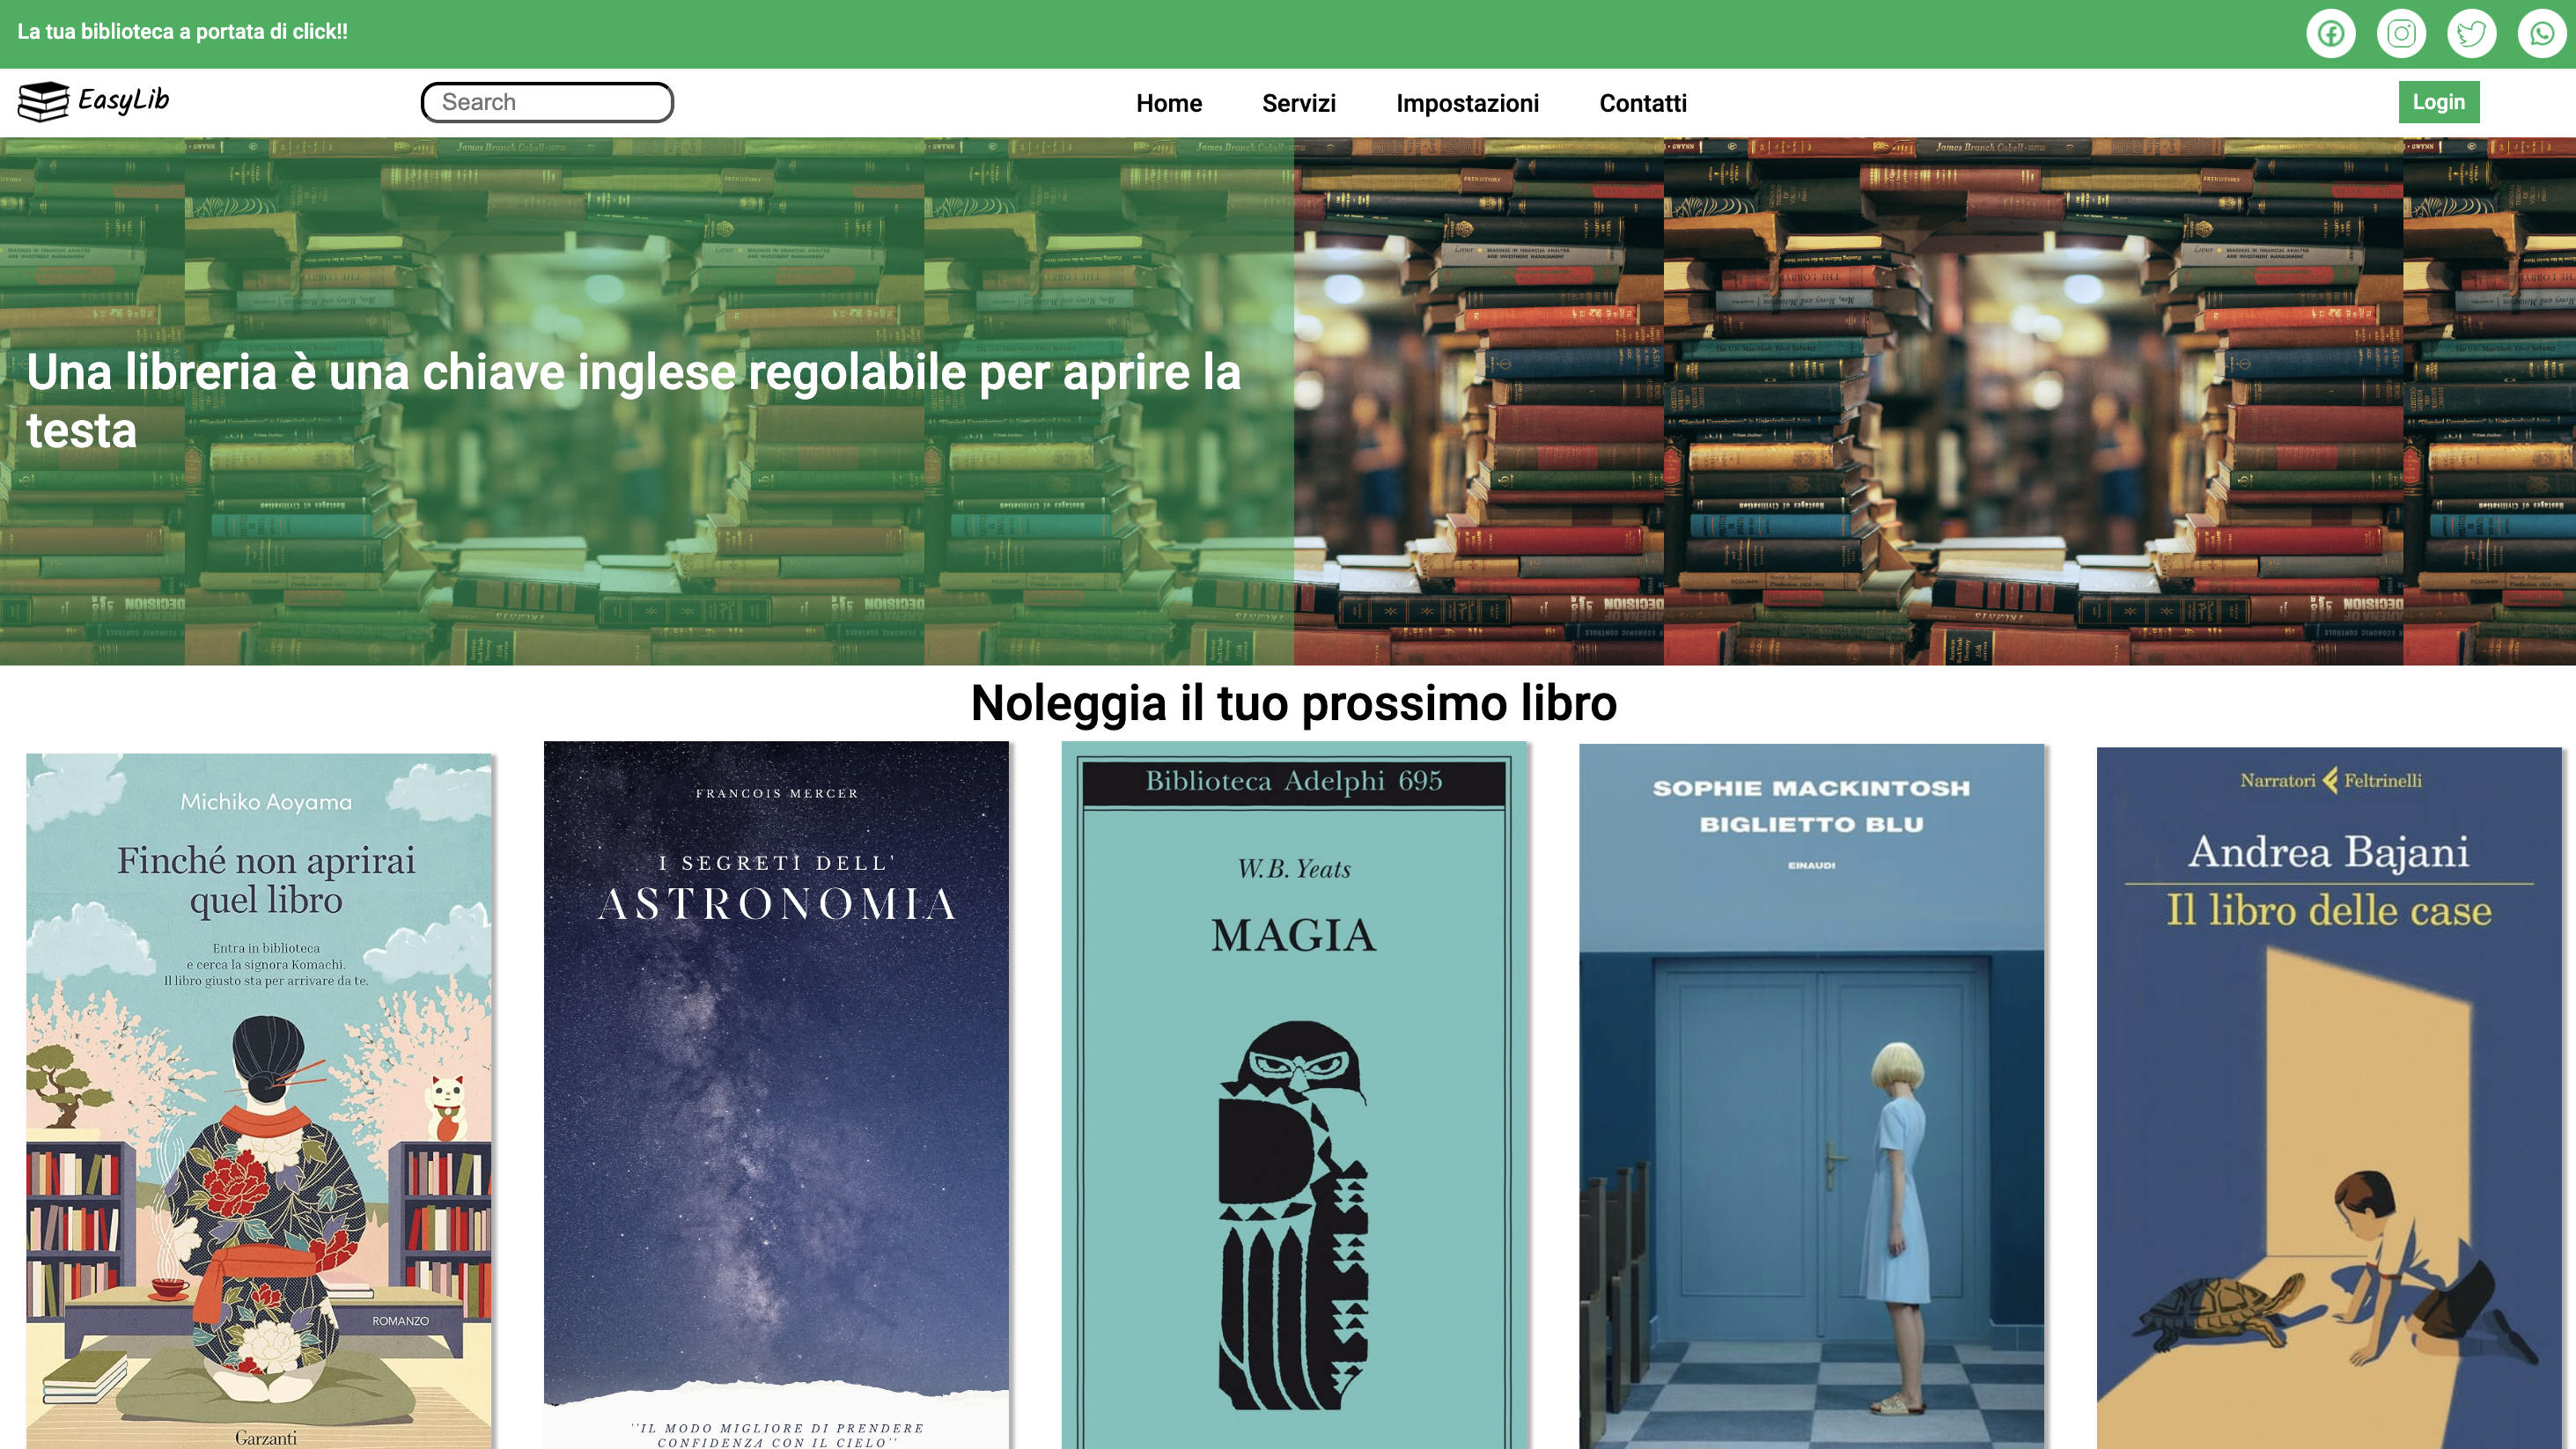
\includegraphics[width=130mm]{D1/Images/Homepage.png}
    \caption{Homepage utente autenticato}
\end{figure}
\subsection{Pagina di Login}
La pagina di login è accessibile cliccando il tasto ‘Login’ presente in alto ad ogni pagina. La pagina alla sua sinistra mostrerà anche un messaggio di ‘Benvenuto’.

\begin{figure}[H]
    \centering
    \includegraphics[width=130mm]{D1/Images/Login.png}
    \caption{Schermata di login}
\end{figure}

\subsection{Pagina di Registrazione}
Se una volta cliccato il tasto ‘Sign In’ l’utente vuole registrarsi per unirsi al sistema bibliotecario, gli sarà fornita la possibilità premendo la scritta ‘Registrati’. Una volta fatto ciò la pagina di login, attraverso un’animazione, diventerà la pagina di registrazione in modo da permettere all’utente di registrarsi.

\begin{figure}[H]
    \centering
    \includegraphics[width=130mm]{D1/Images/Registrazione.png}
    \caption{Schermata di registrazione}
    \label{fig:enter-label}
\end{figure}

\subsection{Archivio}
Una volta che l’utente abbia premuto sul tasto ‘Archivio’ presente nella homepage, verrà aperta una pagina ‘archivio’ nella quale verranno mostrati ulteriori libri disponibili per il noleggio. Premendo il testo ‘Mostra più’ verranno mostrati ulteriori libri, se disponibili.

\begin{figure}[H]
    \centering
    \includegraphics[width=130mm]{D1/Images/Archivio.png}
    \caption{Archivio}
\end{figure}

\subsection{Contatti}
Questa pagina contiene una mappa che fa alla posizione della Biblioteca ed mail e numero di telefono per potersi mettere in contatto con la libreria.

\begin{figure}[H]
    \centering
    \includegraphics[width=130mm]{D1/Images/Contatti.png}
    \caption{Pagina dei contatti}
\end{figure}

\subsection{Impostazioni}
La pagina contiene sulla sinistra diverse scritte, ognuna delle quali porterà alla sezione apposita. In particolare, nel caso di un utente loggato, dovranno essere presenti le sezioni:
\begin{itemize}
    \item Account
    \item I miei noleggi
    \item Le mie donazioni
    \item I miei appuntamenti
    \item Lingua
    \item Notifiche
    \item Pagamenti
    \item Privacy
\end{itemize}

\begin{figure}[H]
    \centering
    \includegraphics[width=130mm]{D1/Images/impostazioni.png}
    \caption{Pagina di impostazioni}
\end{figure}

\subsection{Modulo inserisci Libri in Archivio}
Affinchè possa essere inserito un libro nell’archivio, si dovrà riempire un modulo online nel quale saranno richieste le informazioni necessarie. In particolare verranno richieste le info:
\begin{itemize}
    \item Titolo
    \item Autore
    \item Genere
    \item N° pagine
    \item Editore
    \item EAN
    \item Descrizione
\end{itemize}

\begin{figure}[H]
    \centering
    \includegraphics[width=130mm]{D1/Images/inseriscilibro.png}
    \caption{Modulo Inserisci libro in archivio}
\end{figure}

\section{Design del Back-end}
Nel presente paragrafo vengono elencati i componenti con cui l’applicazione interagirà esternamente e il loro utilizzo, compreso sottostante un semplice diagramma esplicativo (Figura 8).
\subsection*{Gmail API}
La API di Gmail verrà utilizzata per l’accesso all’applicazione e per la ricezione di avvisi riguardanti notifiche in app.
\subsection*{MongoDB}
L’applicazione utilizzerà il database di MongoDB per l’archivio virtuale dei libri della biblioteca e per l’archivio degli utenti verificati.
\subsection*{Paypal API}
Le multe riguardanti libri non restituiti entro il tempo limite verranno pagate tramite l’utilizzo di PayPal.
\subsection*{Google maps API}
Per permettere agli utenti di trovare più facilmente la sede fisica della biblioteca l’applicazione utilizza l’API di Google Maps.

\subsection*{Auth0 API}
Si userà questo servizio che mette a disposizione un sistema di autenticazione per effettuare la registrazione degli utenti e il login. Il sistema Auth0 permetterà di gestire anche il ripristino e
il cambiamento della password.

\begin{figure}[H]
    \centering
    \includegraphics[width=130mm]{D1/Images/backend.png}
    \caption{Diagramma del Back-end}
\end{figure}
\end{document}
